\documentclass[a4paper]{article}
\usepackage{fullpage}
\usepackage{hyperref}
\usepackage{graphicx}
\usepackage{geometry}
\title{Scenario Editor}
%\author{Group 3 of the A Search And Rescue Context Project}
\date{}
\author{}

\geometry{verbose,lmargin=1.5cm,rmargin=1.5cm,tmargin=2cm,bmargin=2cm}
\pagenumbering{gobble}

\begin{document}
\maketitle

\begin{figure}[h]
\begin{center}
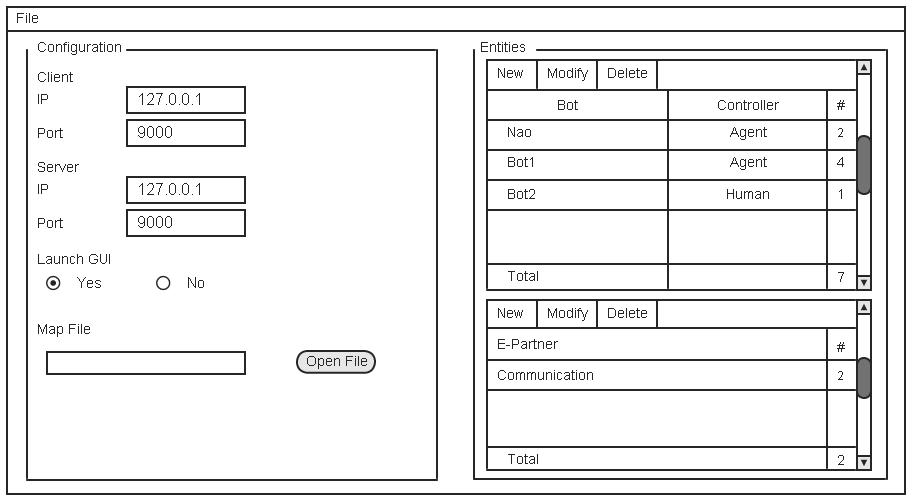
\includegraphics[scale=0.5]{design.jpg}
\end{center}
\caption{The Scenario Editor}
\end{figure}

\section*{General Layout}
This document describes how the Scenario Editor (Figure 1) looks like. When you open the editor, you see two main parts:
\begin{enumerate}
\item The Configuration panel, which is used to create, open and save configuration files.
\item The Entity panel, where a list of the agents and a list of the e-partners is being displayed. Here you can create, modify, rename, duplicate and delete bots.
\end{enumerate}
At the top of the editor you can see a $File$ menu. If you click on that, you get the options to create a new configuration, save your configuration, open a configuration and to exit the editor.

\section*{Configuration}
On the left side of the editor you can configure a scenario as you like. The Client IP, the Client Port, the Server IP and the Server Port should already contain the default values. You can change them if you need to. If you have an Agent class file you want to use, you can import them by selecting the $Open$ $file$ buttons at the right sections.

\section*{Entities}
On the right side of the editor you can create, modify, rename, duplicate and delete entities. There's one list for the agents which enables the user to control the configuration of agents and one list which enables the user to control the configuration of E-partners.
\end{document}